\documentclass[]{scrartcl}

\usepackage{\string~"/LaTeX/StylePackage"}

\title{The Mass Shell}
\author{Florian Bierlage}
\date{\today}


\begin{document}

\maketitle
\newpage
\tableofcontents
\newpage

The mass Shell is a way to illustrate the relation between energy, momentum and mass in relativistic Quantum Mechanics.

\section{The Four Momentum}

In special relativity, you can combine Energy into the momentum vector, and create what is known as the four momentum. It looks like
\begin{equation}
	p = \left[\frac{E}{c}, \vec{p}\right] = \left[\frac{E}{c},p_x, p_y, p_z\right].
\end{equation}
We define the square of the four momentum via the Minkowski metric. We want to say, that
\begin{equation}
	p^2 = p_\mu p^\mu
\end{equation}
where we define
\begin{equation}
	p_\mu = g_{\mu\nu}p^\nu, g_{\mu\nu} = \begin{pmatrix}
		1 & 0 & 0 & 0\\
		0 & -1 & 0 & 0\\
		0 & 0 & -1 & 0\\
		0 & 0 & 0 & -1\\
	\end{pmatrix}
\end{equation}
where $g_{\mu\nu}$ is called the metric tensor for the minkowski metric. one important thing is that some people will define the Minkowski metric as defined here, where the diagonal is in the form of $(+, -, -, -)$ but some might define it as $(-, +, +, +)$.

Now, knowing how we define our \textbf{contravariant} momentum $(p_\mu)$, we can calculate it, and with it the square of the momentum.
\begin{equation}
	p_\mu = g_{\mu\nu}p^\nu = \left[\frac{E}{c}, -\vec{p}\right] \rightarrow p_\mu p^\mu = \left(\frac{E}{c}\right)^2 - |\vec{p}|^2.
\end{equation}
The magnitude of the Four momentum is
\begin{gather}
	E^2 = (|\vec{p}|c)^2 + (mc^2)^2 \rightarrow \left(\frac{E}{c}\right)^2 = |\vec{p}|^2 + (mc)^2 \rightarrow \left(\frac{E}{c}\right)^2 - |\vec{p}|^2 = (mc)^2\\
	\Rightarrow |p| = \sqrt{(E/c)^2 - |\vec{p}|^2} = mc,
\end{gather}
so we can also say that
\begin{equation}
	p^2 = (mc)^2 = \left(\frac{E}{c}\right)^2 - |\vec{p}|^2.
\end{equation}.
While, depending on the Inertial frame that the particle is being observed from, the momentum and the energy of the particle may differ, both the rest mass $m$ and the speed of light $c$ are the same in every inertial frame, which means that the magnitude of the momentum (Eq. 6) and the magnitude of its square (Eq. 4) are constant.

\newpage
\section{The Mass Shell}

From our previous work we can now define a relation between Energy and momentum, involving mass, where in a one Dimensional example with $p_y = p_z = 0$ Energy $E$ is the y axis and momentum $p_x$ is the x axis. Then we have the relation
\begin{equation}
	\frac{E}{c} = \sqrt{(mc)^2 + |p_x|^2}
\end{equation}
This can then also be done with not just $p_x$ but also $p_y$ and $p_z$, where a graph with all momentums would be extremely hard to visualize.

\begin{figure}[h]
	\centering
	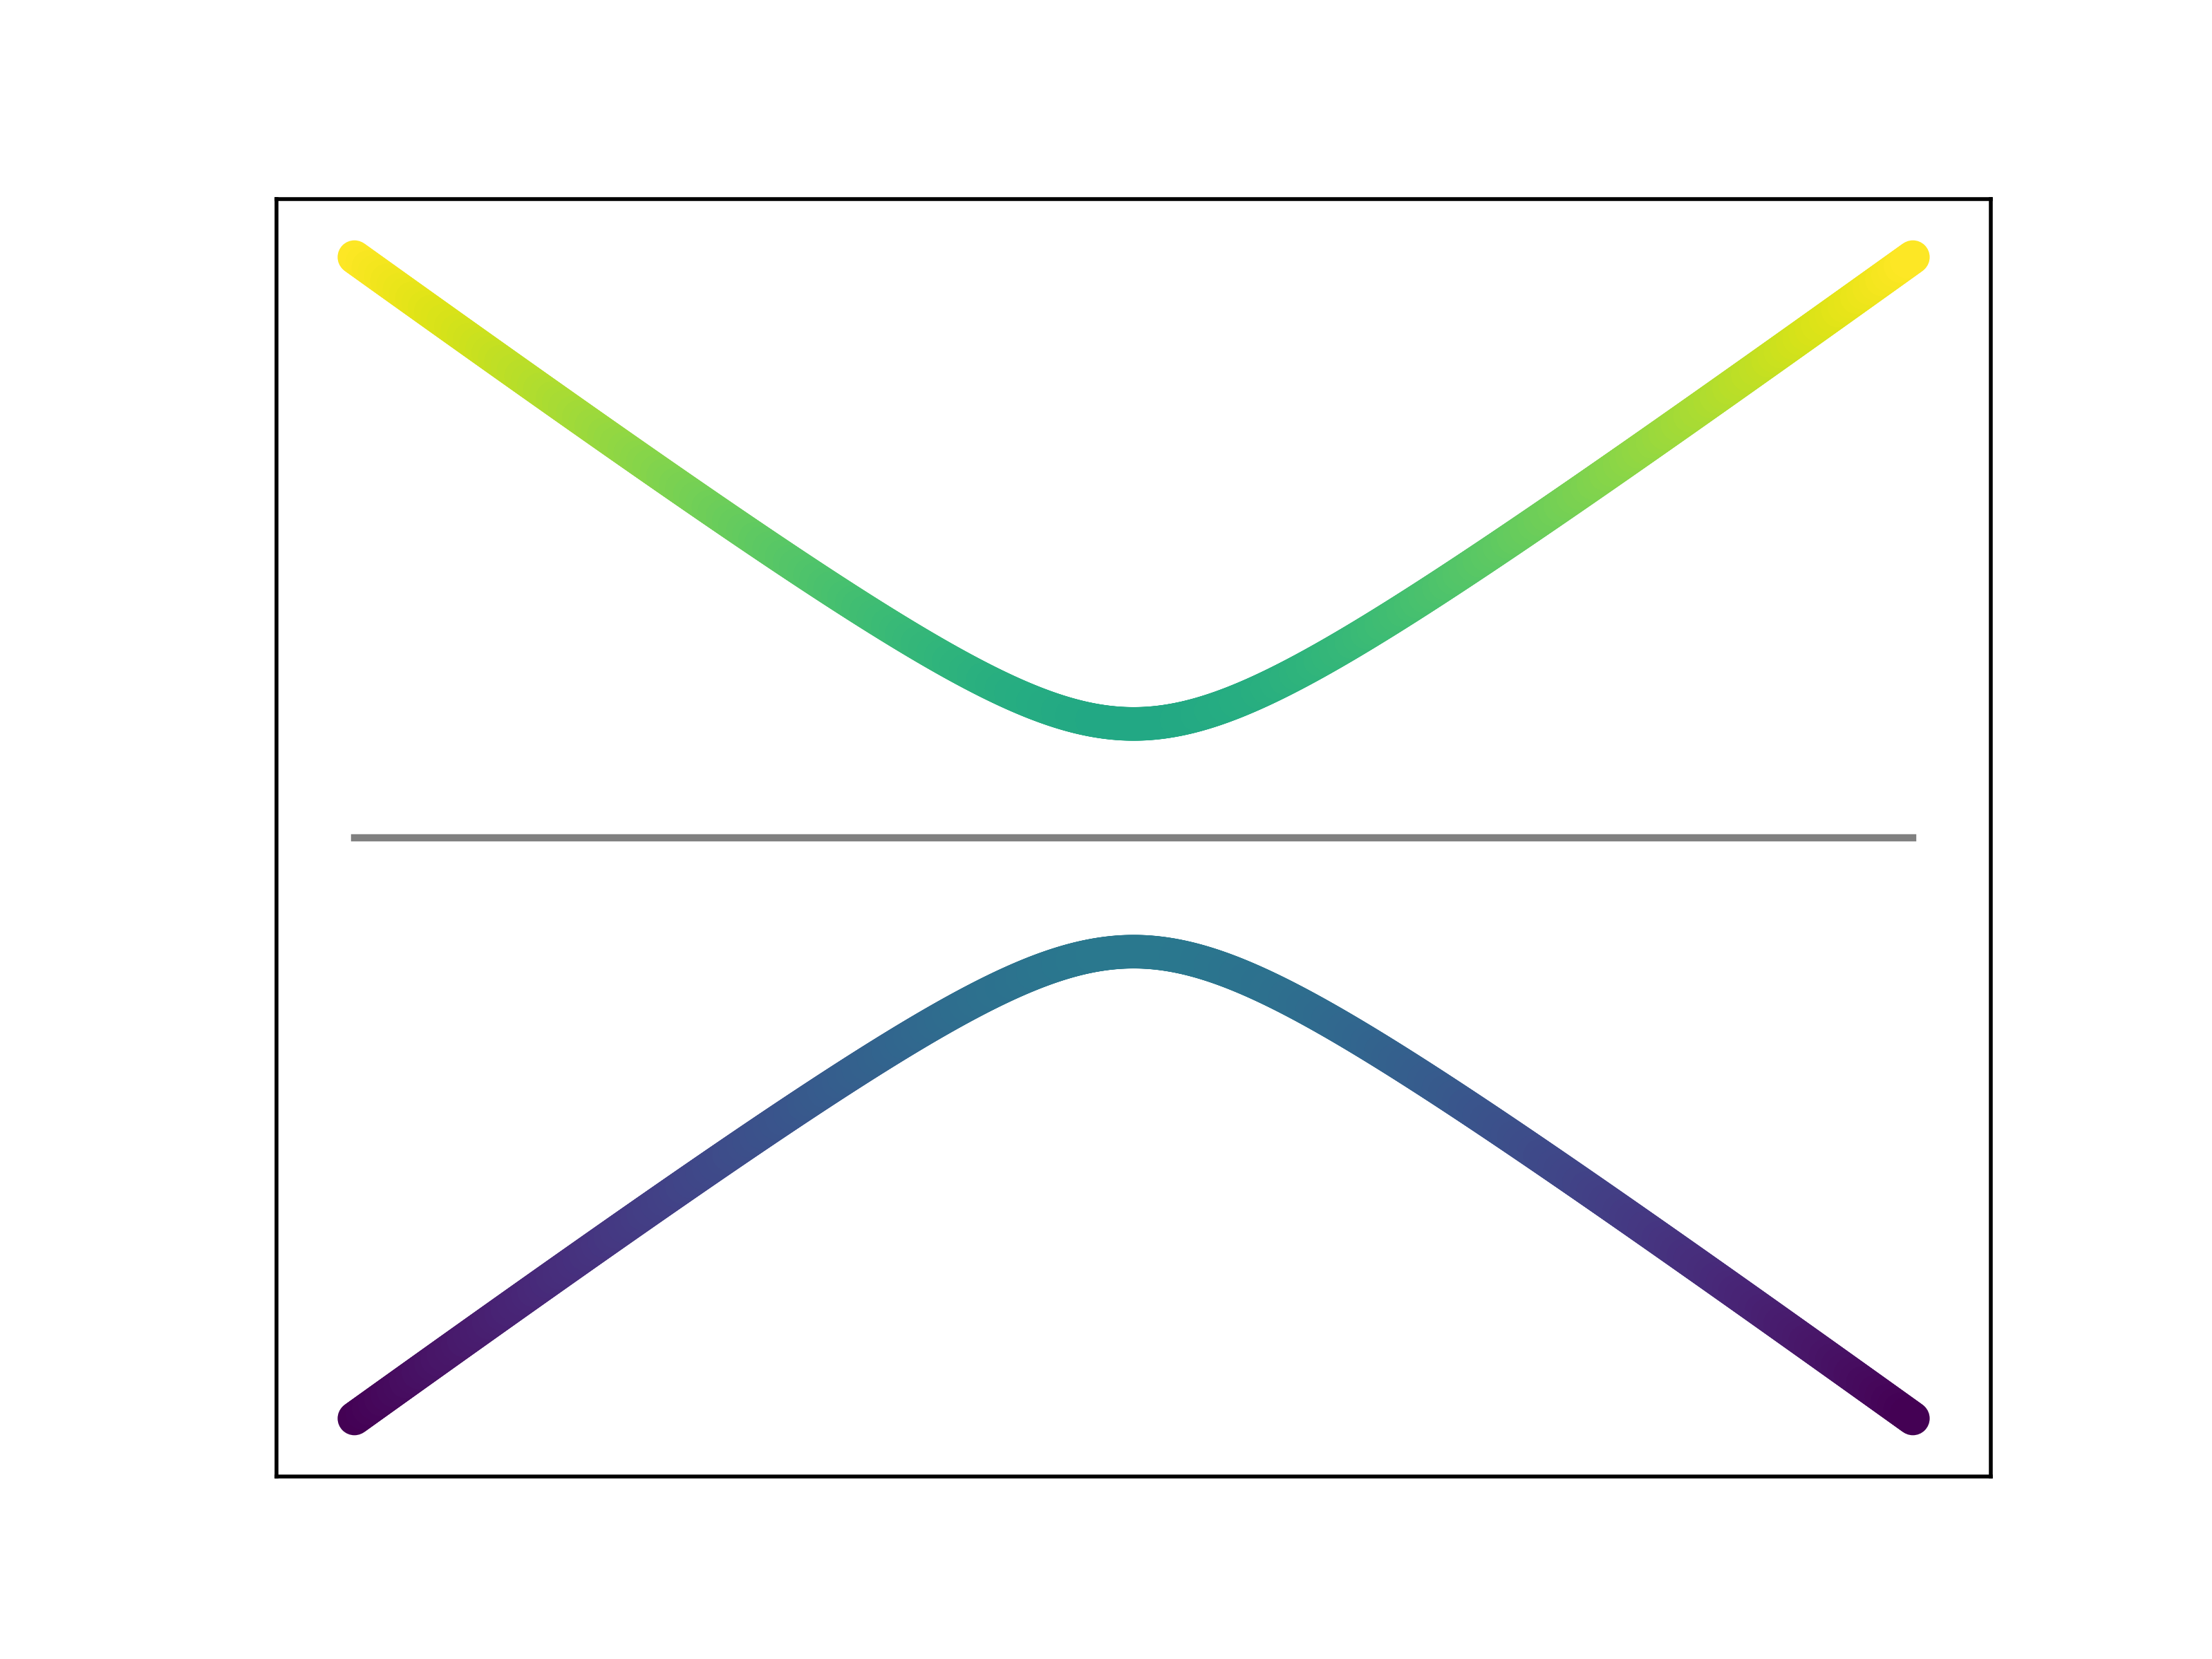
\includegraphics[scale=0.8]{2DMassShell}
	\caption{2D plot of the mass shell with only variable px}
\end{figure}\newpage
\begin{figure}[H]
	\centering
	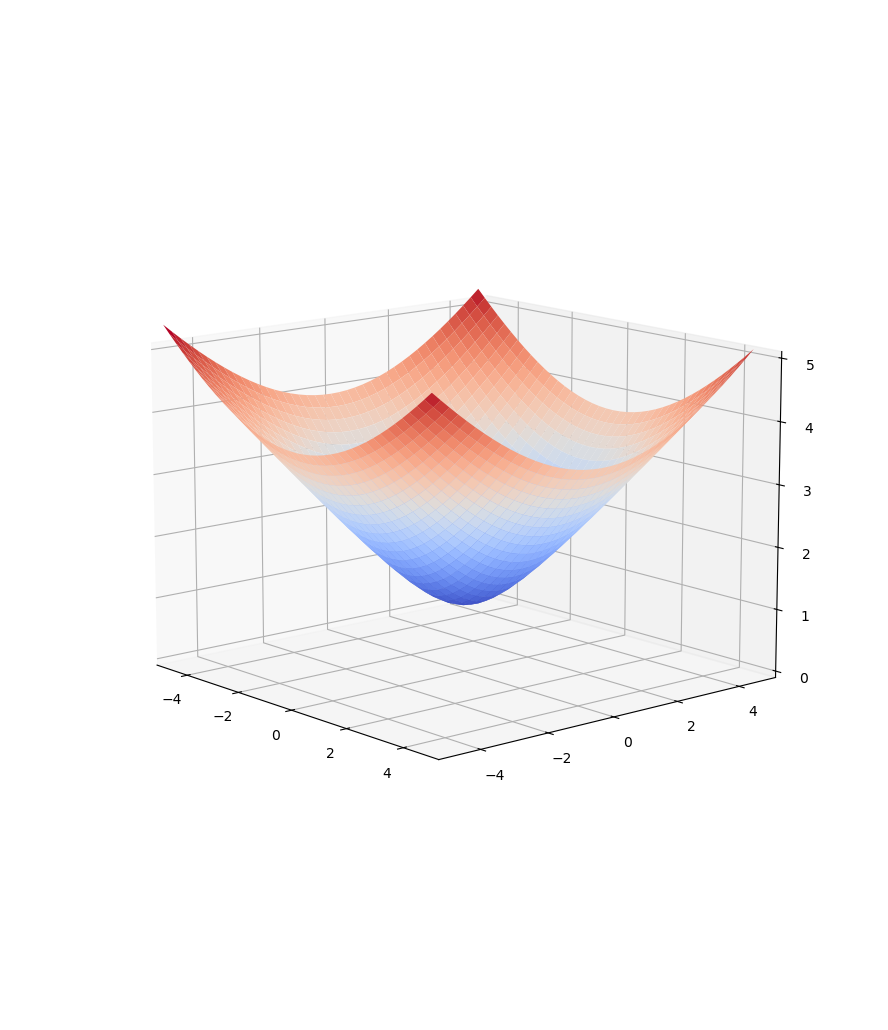
\includegraphics[scale=0.6]{3DMassShell}
	\caption{3D plot of the mass shell with only variables px and py}
\end{figure}
\newpage
Shown in the 2D plot is $\frac{E}{c}$ plotted against $\sqrt{(mc)^2 + p_x^2}$ and in the 3D plot the same with $\sqrt{(mc)^2 + p_x^2 + p_y^2}$. Something to note is that the negative values which you can see in the 2D plot also exist in the 3D plot, but aren't shown.

Also important is seeing that for $p_x = p_y = 0$, $E/c = mc$. This makes sense, as the energy mass relation given by Einstein tells us that for a particle at rest $E = mc^2$. The whole Shell also changes with the mass of the particle, for example for a particle with zero mass, the 2D mass shell would just be $E/c = p_x$.

Going back to the negative plot in the 2D mass shell, this comes from the fact that if we take the square root of a number it will give us a negative and a positive number. $1 = (-1)^2 = 1^2$.\\\\\\
The importance of this shell is that only the particles which lie on it may exist, meaning that when you integrate over the four momentum, you may only want to select the particles on the mass shell, like this
\begin{equation}
	\varphi(x) = \int \frac{d^4p}{(2\pi)^4}e^{-p\cdot x}C(p)\delta\left((p^0)^2 - |p|^2 - m^2c^2\right)
\end{equation}



\end{document}

